% (f) Popis implementace/realizace produktu se zaměřením na nestandardní části řešení.

\chapter{Realizace}
% Popis implementace/realizace se zaměřením na nestandardní části řešení.
Během implementace (\textit{implementation}) se objevila celá řada zádrhelů, z nichž mnoho souviselo s doposud ne zcela zdokumentovanými a odladěnými technologiemi, přesto pro mne byla realizace velmi přínosná -- neustálým hledáním různých řešení a alternativ jsem nutně narazil na mnoho dalších zajímavých postřehů a nápadů. Kapitola se zabývá řešenými problémy, komplikacemi a implementací bezpečnosti. % , potenciální aplikací v ideálním světě

\section{Serverová aplikace}
Když se zpětně ohlížím za implementací serverové aplikace, náročná objektivně vůbec nebyla, osobně jsem ale žádnou z používaných technologií / knihoven\dots v té době neznal, takže mi náročnost přišla enormně vysoká. Rozsah popisu realizace serverové aplikace je tak krátký -- mnoho objektivně zajímavých míst se v ní nevyskytlo.

Realizováno bylo pouze zpracování čtyř rozličných typů zdrojů -- implementace ostatních by byla dlouhotrvajícím opakováním stejných postupů a práci by moc neobohatila.

\subsection{Řešené problémy}
V době, kdy byl vytvořený návrh, bylo vytvoření aplikace už poměrně snadné. Popíšu tedy jen ve stručnosti několik základních částí řešení.

\subsubsection{Zpracování zdroje}
Proces zpracování zdroje je poměrně přímočarý. Nejprve je zdroj po jednotlivých \textit{chuncích} stažen následně sestaven:
\begin{verbatim}
var http = require('http'); //načtení modulu

var request = http.get({
    host: 'akce.cvut.cz',
    path: '/index.php'
});
request.on('response', function (r) {
    var data = '';
    r.on('data', function (chunk) {
        data += chunk;
    });
    r.on('end', function () {
        //zpracování dat
    });
});
\end{verbatim}
Poté je pro snadnou a spolehlivou manipulaci vytvořen model dokumentu daného formátu, se kterým se pak pracuje, například pro \glsname{HTML} nebo \glsname{XML}:
\begin{verbatim}
var $ = require('jquery');
var jqo = $(data);
jqo.find('#content span.location').text();
\end{verbatim}
Pro iCalendar:
\begin{verbatim}
var icalendar = require('icalendar');
var ical = icalendar.parse_calendar(data);
ical.events()[0].properties.LOCATION;
\end{verbatim}
Získaná data jsou pak ukládána do grafového úložiště:
\begin{verbatim}
var rdfstore = require('rdfstore');

var store = rdfstore.create(config, function (store) {
    var graph = store.rdf.createGraph();

    store.rdf.setPrefix(
        "lode", "http://linkedevents.org/ontology/");

    for (var e in ical.events()) {
        var event = store.rdf.createNamedNode(
            ical.events()[e].properties.URL.value);

        graph.add(
            store.rdf.createTriple(
                event,
                store.rdf.createNamedNode(
                    store.rdf.resolve("rdf:type")),
                store.rdf.createNamedNode(
                    store.rdf.resolve("lode:Event"))
            )
        );

        //další informace zpracovávány obdobně
    }

    store.insert(graph, function () {
        console.log("Graph has been inserted.")
    });
});
\end{verbatim}
Zdrojový kód je v tomto případě dobře čitelný, žádné další komentáře tedy asi nepotřebuje. Za povšimnutí pouze stojí asynchronní charakter celé aplikace -- nikde se neblokují zdroje zbytečně a nemůže se stát, že by nějaká událost předběhla jinou.

\subsubsection{Zdroje uživatelských jmen}
Nepodařilo se mi nalézt vhodný zdroj uživatelských jmen vyučujících a neakademických pracovníků. Zatímco uživatelská jména studentů jsou zveřejněna na \url{https://timetable.fit.cvut.cz/public/cz/studenti/}, na obdobné stránce věnované učitelům, \url{https://timetable.fit.cvut.cz/public/cz/ucitele/}, jsou pouze tituly, křestní jména a příjmení -- tedy nic, co by bylo vhodným identifikátorem. Zdroj uživatelských jmen neakademických pracovníků se mi nepodařilo nalézt žádný. Vzhledem k plánovanému budoucímu napojení aplikace na KOSapi (\url{http://kosapi.fit.cvut.cz/}), až získá přístup do \glsname{KOS}, byly jako dočasné řešení zvoleny soubory obsahující jména a uživatelská jména všech osob.

\subsubsection{Routování}
Aplikace je serverem\footnote{Pozor, zde je důležité vzít v potaz vymezení pojmů z poznámky \ref{fnt:aplikace} na straně \pageref{fnt:aplikace} -- aplikace, o které je řeč, je \textit{serverovou aplikací} v užším slova smyslu -- není nazývána \textit{serverovou aplikací} proto, že by nutně musela být serverem, ale proto, že je jednou z komponent serverového řešení. Že je tedy také serverem je pouze shoda náhod.} a obsluhuje se \glsname{HTTP} požadavky, je tak dosaženo větší univerzálnosti. Například pro aktualizaci osob spjatých s fakultou je třeba odeslat požadavek \texttt{GET} na \glsname{URL} \texttt{http://\linebreak[0]localhost:1337/\linebreak[0]osoby/}, na které je server spuštěný. Zpracování takového požadavku je vyřízeno následujícím kódem ze \textit{spouštěcího} souboru aplikace:
\begin{verbatim}
var express = require('express'); //načtení frameworku express

var app = express.createServer(); //vytvoření serveru

app.get('/osoby/:login?', function (req, res) {
    require('./sources/usermap.js').process(req.params.login);
    res.send("OK: Source enqueued for processing.");
});

//další zdroje zpracovávány obdobně

app.get('*', function (req, res) { //neodchycené cesty
    res.send("Error: Service not found.", 404);
});

app.listen(1337); //spuštění aplikace na portu 1337
\end{verbatim}
V těchto několika řádcích je vytvořený celý server zpracovávající příchozí požadavky. Na pátém řádku je řečeno, že cesta směřující do \textit{segmentu} osoby bude touto metodou odchycena. Odchycen bude i další, nepovinný, segment, který bude uložený do proměnné \texttt{login}. Je tedy možné volat i \glsname{URL} \texttt{http://\linebreak[0]localhost:1337/\linebreak[0]osoby/\linebreak[0]molnaja2/}, aniž by došlo k odchycení dvanáctým řádkem, který klientovi vrátí patřičnou chybu.

Uvnitř metody je na prvním řádku vyžadováno zavolání metody \texttt{process()} z uvedeného souboru s parametrem \texttt{login}. V této metodě je na základě přítomnosti parametru rozhodnuto, jestli se mají zpracovat všechny osoby nebo jen jedna konkrétní. Na druhém řádku je klientovi odesláno oznámení o úspěšném přijetí požadavku.

\subsubsection{Nastavení časovače}
Vzhledem k výše uvedené obsluze \textit{serverové aplikace} \glsname{HTTP} požadavky je možné časovač reprezentovaný cronem jednoduchým nastavením, například:
\begin{verbatim}
# aktualizace jidelnicku kazdy den 3 minuty po zverejneni
3 9,10,16,17 * * * user curl localhost:1337/jidelnicky/\
               2>&1 1> jidelnicky.all.log 2> jidelnicky.err.log

# aktualizace osob kazdy den 10 minut po druhe hodine
10 2 * * * user curl localhost:1337/osoby/\
               2>&1 1> osoby.all.log 2> osoby.err.log

# aktualizace akci 10 minut po kazde sude hodine
10 */2 * * * user curl localhost:1337/akce/\
               2>&1 1> akce.all.log 2> akce.err.log

# aktualizace rozvrhu kazdy den 10 minut po druhe hodine
10 2 * * * user curl localhost:1337/rozvrh/\
               2>&1 1> rozvrh.all.log 2> rozvrh.err.log
# aktualizace rozvrhu v dobe tvorby 10 minut po kazde hodine
10 * * 6,9,10,1,2 * user curl localhost:1337/rozvrh/\
               2>&1 1> rozvrh.all.log 2> rozvrh.err.log
\end{verbatim}
Prvních pět parametrů udává čas vykonání akce (minuta, hodina, den měsíce, měsíc, den týdne), šestý uživatele, zbytek je vykonání příkazu -- odeslání požadavku a zalogování výsledku.

% \subsection{Implementace bezpečnosti}

\subsection{Komplikace}
Během implementace serverové aplikace vyvstalo několik komplikací, které bylo třeba vyřešit:

\subsubsection{Převod kódování}
Node.js vznikl až po prosazení \glsname{UTF}-8, dá se tedy předpokládat, že bude toto kódování podporovat. Předpoklad je to samozřejmě, i dle dokumentace \cite{NodeEncoding}, správný; horší je to ale, dle stejného zdroje, s ostatními kódováními. Samotný Node.js může data v nich převádět do \textit{bufferu}, který pak lze následně, například pomocí systémového programu iconv volaného prostřednictvím knihovny node-iconv, převést do správného kódování.

Problém vyvstává u vysokoúrovňových nástrojů, které například dokáží jednoduše stáhnout cizí internetovou stránku a předpřipravit ji k následnému zpracování -- pokud je u těchto nástrojů vrácen třeba \glsname{DOM}, v případě, že pocházela stránka ze zdroje, který využíval s Node.js nekompatibilní kódování, řekněme Windows-1250, převod kódování už nelze zpětně ovlivnit. Při zpracovávání některých stránek jsem tak musel zůstat u nízkoúrovňových nástrojů.

\subsubsection{Špatně formované XML}
Při práci se sémantickým úložištěm rdfstore-js jsem narazil na špatně formované \glsname{XML}. Chybu jsem identifikoval -- jednalo se o sekvenci \verb|<literal>>| v některých případech generovaného \glsname{XML}, nalezl chybu v kódu, nahlásil a odeslal \textit{patch}. V současné době je chyba již odstraněna \cite{IssueLiteral}.

% \subsection{Ideální implementace}


\section{Mobilní aplikace}
Pod pojmem \textit{mobilní aplikace} se skrývá aplikace pevně nezávislá na výše uvedené \textit{serverové}. Jejím hlavním cílem je sloužit studentovi \glsname{FIT} \glsname{CVUT} jako průvodce, zároveň má ale plnit i účel ukázky využití \glsname{SPARQL} endpointu vytvořeného v \textit{serverové} části.

\subsection{Řešené problémy}
Implementace mobilní aplikace přinesla mnoho menších problémů, které bylo třeba vyřešit. Mezi nejzajímavější patří:

\subsubsection{Vyhledávání v navigaci}
Aby bylo vyhledávání pro uživatele co nejvíce přívětivé, je třeba mu věnovat hodně pozornosti. Změnou vyhledávací fráze (stiskem klávesy, stiskem vyhledávacího tlačítka, odesláním formuláře, změnou formuláře) je vyvoláno hledání, kde jsou nejprve z vyhledávané fráze ořezány (počáteční a koncové) bílé znaky a následně je převedena do dvou regulárních výrazů -- první je tvořený frází tak, jak je zadána, druhý je normalizovaný. Normalizací je odstraněna diakritika, interpunkce a zbylé bílé znaky. Nyní už jsou prohledána všechna místa z databáze, nejprve na přítomnost prvního zmiňovaného regulárního výrazu, poté se normalizují a testují na druhý regulární výraz. Ve vyhledávání nezáleží na velikosti písmen.

V průběhu celého procesu jsou zpracovávány krajní situace a řešena otázka uživatelské přívětivosti -- v případě chyby v regulárním výrazu je uživateli nabídnuta oprava, jsou vypisována hlášení o průběhu vyhledávání a dle počtu nalezených výsledků jsou tyto prezentovány -- jediný výsledek je rovnou zobrazen, více výsledků se vypíše a uživatel má možnost si dále z nich vybrat, případně pokračovat v zadávání hledané fráze.

\subsubsection{Mapa v navigaci}
Mapa v navigaci je tvořena \glsname{SVG} obrázkem, se kterým je manipulováno JavaScriptem. Z mapy je zobrazována pouze výseč, která je navíc dle potřeby škálována -- to nutně vede k mnoha různým algoritmům:
\begin{itemize}
 \item Změna velikosti mapy v případě změny velikosti okna (minimalizací prohlížeče nebo třeba překlopením mobilního zařízení) -- velikost mapy se totiž automaticky nastavuje na velikost obrazovky, aby nebyla zbytečně velká a přesto ji mohl mít uživatel zobrazenou na celém displeji.
 \item Posun zobrazované výseče po vyžádání uživatelem nebo na nalezený objekt. Je nutné brát v potaz aktuální škálování mapy.
 \item Škálování mapy vyžádané uživatelem nebo dle nalezeného objektu. Je nutné brát v potaz aktuální zobrazovanou výseč.
 \item Zjištění pozice vykonaného gesta -- je odvozována na základě pozice obalového elementu, zjišťování pozice z mapy dávalo vlivem různých implementací jiné výsledky napříč prohlížeči.
 \item Převedení zeměpisných souřadnic na místo na mapě.
\end{itemize}

% \subsubsection{Optimalizace}
% vyhledávání

\subsubsection{Rozdílné DOM u HTML a SVG}
\glsname{SVG} je, co se týče návrhu \glsname{DOM}, komplikovanější, než \glsname{HTML} -- zatímco u \glsname{HTML} stačí k hodnotě atributu v \glsname{DOM} přímo přistoupit, v \glsname{SVG} se musí zpravidla ještě o dvě úrovně níže, tedy třeba místo k \texttt{.width} se musí přistupovat k \texttt{.width.baseVal.value}. Při implementaci to bylo třeba brát v potaz.

\subsubsection{Malá velikost displeje}
Ačkoliv je toto omezení u mobilních zařízení zřejmé, nic to nemění na faktu, že se s ním musí neustále počítat a je třeba vybírat vhodné komponenty a ty vhodně rozvrhovat. Malá velikost displeje byla omezením i z opačného hlediska -- prsty jsou u dotykových telefonů, vzhledem k velikosti displeje, poměrně velké a ovládací prvky tak musí být dostatečně rozměrné, což konzumuje další místo. Mým cílem proto bylo vizualizovat jen to nejnutnější.

\subsubsection{Různé typy polohovacích zařízení}
Různá zařízení poskytují různé ovládací prvky využívající různé principy, aplikaci je ale potřeba přizpůsobit pro všechny najednou. Jiné je ovládání pro myš (touchpad, trackpad), jiné pro klávesy a jiné pro dotyková zařízení -- právě s těmi je problém -- v rámci použitých technologií ještě nebyl vytvořen žádný standard pro zpracování zpracování gest, proto bylo nutné umístit nad mapu výrazné ovládací prvky.

\subsubsection{Dynamické načítání lokálních souborů}
Z bezpečnostních důvodů došlo v minulosti v prohlížečích k zamezení načítání jakýchkoliv souborů, mimo JavaScriptu, z jiných zdrojů, než ze kterých stránka pochází. To v některých případech\footnote{Příkladem je Google Chrome a jeho základ Chromium \cite{BugChromeOrigin}.} přerostlo v zamezení dynamického načítání jakýchkoliv lokálních souborů -- jejich zdroj nemá žádnou hodnotu (\texttt{null}), takže je nelze načíst. Aby byla zachována možnost offline využití aplikace na větší skupině zařízení, byla aplikace přepsána na jediné možné řešení -- explicitní uvedení všech potenciálně vkládaných souborů, což značně omezilo modularitu aplikace.

Například v případě \glsname{SVG} je široká nabídka volby -- lze vložit JavaScriptem do elementů \texttt{img} (\texttt{<img src="map.svg"\ />}), \texttt{embed} (\texttt{<embed src="map.svg"\ />}), \texttt{object} (\texttt{<object type="image/svg+xml"\ data="map.svg"\ />}), \texttt{iframe} (\texttt{<iframe src="map.svg"\ />}), pokud je pak umožněna manipulace s obsahem pomocí JavaScriptu, tak jen velice neohrabaně. Další možností je vložit \glsname{SVG} přímo do \glsname{HTML} kódu -- v případě dynamicky generovaného kódu by bylo vhodné celý soubor načíst a na místo vložit, jenže zde narážíme na problém z předchozího odstavce -- některé prohlížeče to neumožní. Zbývá tedy poslední řešení -- celý soubor převést do JavaScriptového řetězce, uložit do proměnné a vložit z ní. Jedině tak zle vložit do stránky \glsname{SVG} soubor, aby s ním pak bylo snadné manipulovat prostřednictvím jediného \glsname{DOM}.

% \subsubsection{Otevírání lokálních souborů}
% Omezení zmíněná v předchozím odstavci stupňuje až do extrémů mobilní prohlížeč Chrome Beta, který nepovolí ani přímé otevření lokálního souboru. \todo{Ověřit, možná nefunguje celé Chrome\dots}

\subsubsection{Zpracování Cross-Origin zdrojů}
\label{sec:mobil:cross-origin}
Aplikace potřebuje získávat a zpracovávat cizí zdroje -- aby poskytovala aktuální informace, nevystačí si jen s lokálním úložištěm, musí přímo k jejich původci. To je ale zpravidla v doméně použitých technologií komplikované -- webové prohlížeče z bezpečnostních důvodů nepovolují k cizím zdrojům přístup (výjimkou je například JavaScript -- více dále), takže je třeba danou situaci řešit.

\glsname{SPARQL} endpoint ze serverové aplikace, tedy hlavní předpokládaný zdroj informací, máme plně ve své režii, takže na něm můžeme povolit \gls{CORS}, tedy technologii umožňující serveru zpřístupnit své zdroje i z jiné domény. Jediný problém je u špatné podpory některých prohlížečů.

Z již dříve popsaných důvodů, tedy malého rozsahu sémantické databáze, ale finální aplikace podporuje mimo přístupu k samotnému \glsname{SPARQL} endpointu i přímý přístup k původním zdrojům. Zde vyvstává problém -- na cizích zdrojích \glsname{CORS} povolit nemůžeme, je tedy třeba najít jiné řešení. Tím je \gls{JSONP}, tedy postup umožňující získat přes JavaScriptový soubor (ten má výjimku) data ve formátu \glsname{JSON} obalená funkcí námi zvoleného jména, která je po stažení zdroje v prohlížeči vykonána, a tím jsou aplikaci předána data ke zpracování.

\glsname{JSONP} sám o sobě ale nic nevyřeší -- je k němu stejně tak potřeba mít uzpůsobený server. Tady nám pomůže jednoduchá \textit{proxy}, které zadáme požadavek na zdroj, ona ho získá a odešle nazpátek. I zde by nakonec nemuselo být \glsname{JSONP}   potřeba, proxy zase bude v naší režii, v případě existence jiné vhodné, v cizí, a šlo by použít \glsname{CORS}, protože se ale jedná o dočasné řešení v době, kdy ještě některé menšinové prohlížeče \glsname{CORS} nepodporují, rozhodl jsem se si vyzkoušet implementaci další technologie.

Z veřejně k použití dostupných proxy lze využít například server Yahoo! využívaný pro \textit{Yahoo! Query Language} (\url{http://developer.yahoo.com/yql/}) -- na něm je založeno jQuery rozšíření cross-domain-ajax (\url{https://github.com/padolsey/jQuery-Plugins/}), dále je možné na vlastním serveru použít nějaké hotové řešení, například \textit{AJAX Cross Domain} (\url{http://www.ajax-cross-domain.com/}), nebo si vše od základu vytvořit sám.

Rozhodl jsem se pro třetí možnost -- veřejně dostupná řešení nenabízejí potřebné možnosti konfigurace, mezi již hotovými řešeními se mi nepodařilo nalézt vhodné pro konkrétní použití, takže jsem si vytvořil proxy vlastní.\footnote{Byla tedy přidána další serverová aplikace do již tak terminologicky složité situace. Z tohoto důvodu se u zmíněného serveru držím označení \textit{proxy}.}

Proxy je požádána o zprostředkování zdroje, na základě \textit{whitelistu} je rozhodnuto o jeho poskytnutí -- z bezpečnostních důvodů je zamezen přístup ke všem mimo nutně potřebných serverů. Zdroj proxy stáhne, převede na přednastavené kódování -- v rámci JavaScriptu nejsou převody snadné, dojde tak k výraznému usnadnění mobilní aplikaci, a před odesláním odpovědi je zdroj pročištěn -- za využití knihovny \textit{HTML Purifier} je zdroj zvalidněn a je z něj odstraněno vše, co není explicitně dalším \textit{whitelistem} povoleno -- skripty, obrázky, rámce, další zdroje, potenciálně škodlivé atributy a elementy\dots V případě chyby je uživateli (mobilní aplikaci) navráceno příslušné chybové hlášení.

\subsubsection{Uživatelské rozhraní}
Tvorba uživatelského rozhraní mobilní aplikace nepřinesla, mimo tvorby mapy a zpracování cizích zdrojů, žádné zvlášť komplikované úkony. Tvorba mapy byla již popsána. Zpracování cizích zdrojů bylo vyžadováno pro jejich různorodost -- každý poskytoval informace v jiném formátu, transformoval jsem je tedy do obdobnějších reprezentací vhodných pro mobilní zařízení. Pro ilustraci přikládám obrázek \ref{fig:mobil:android:pruvodce} znázorňující uživatelské rozhraní mobilního průvodce.
\begin{figure}[h]
 \centering
 \setlength\fboxsep{0pt}
 \setlength\fboxrule{0.5pt}
 \fbox{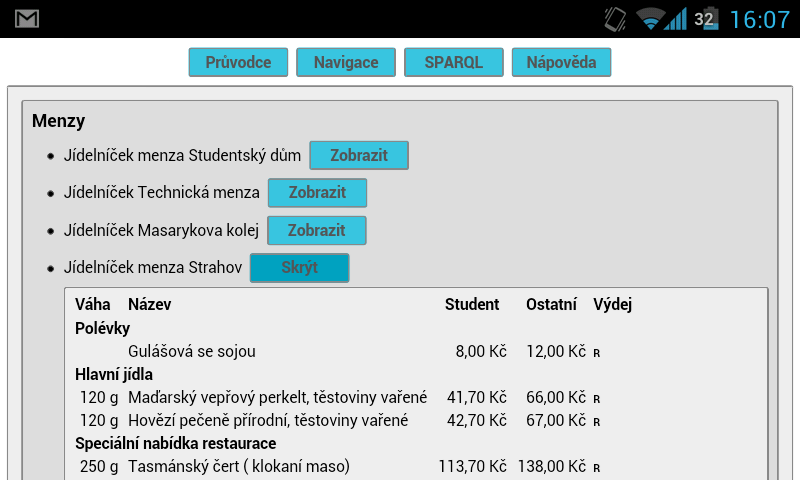
\includegraphics[width=9.1cm]{./figures/android-pruvodce.png}}
 % android-pruvodce.png: 800x480 pixel, 72dpi, 28.22x16.93 cm, bb=0 0 800 480
 \caption{Snímek obrazovky aplikace v prohlížeči platformy Android}
 \label{fig:mobil:android:pruvodce}
\end{figure}



\subsection{Komplikace}
Během implementace mobilní aplikace se objevily i komplikace, mimo očekávaných, již zmíněných v předchozí části, mezi ně patřilo:

\subsubsection{Chyby prohlížečů v implementaci specifikací}
Při práci jsem několikrát narazil na situaci, kdy určitá vlastnost v jednom prohlížeči fungovala, ve druhém nikoliv, a přesto bylo vše implementované správně podle specifikace. V takovém případě pak bývala chyba na straně prohlížeče, který určitou specifikaci špatně implementoval. Situace nastávala převážně u hodně specifických případů. Příkladem může být chybějící podpora pro nastavení transformace \glsname{SVG} elementu JavaScriptem (nutné pro práci s mapou) v prohlížeči Google Chrome \cite{BugChromeTran}, tento problém ale lze obejít vlastním sestavením hodnoty celého atributu a přímým vložením. 

\subsubsection{Implementace SVG}
Implementace \glsname{SVG} je v desktopových prohlížečích na velmi dobré úrovni již nějakou dobu,\footnote{Posledním významným desktopovým prohlížečem podporujícím \glsname{SVG} se stal s dlouhým odstupem verzí 9.0 Internet Explorer \cite{CanIUse}, předtím pro něj ale byly dostupné vhodné pluginy.} v nedávné minulosti se ale podpora značně zlepšila i na poli mobilních zařízení \cite{CanIUse}.

U mobilních zařízení nepřekvapuje chybějící implementace některých neklíčových možností \glsname{SVG}, jako je třeba průhlednost v případě Opery Mobile. V této oblasti v současné době rozsáhlému nasazení nepřeje \glsname{SVG} nepodporující hojně využívaný nativní webový prohlížeč Androidu verze 2, od verze 3 je podpora zavedena. Problém lze obejít využitím jiného dostupného prohlížeče.

Překvapením byla pomalá, ačkoliv jinak velmi rozsáhlá, implementace \glsname{SVG} v prohlížeči Mozilla Firefox -- po některých operacích, v mém případě to byla třeba změna hodnot atributu \texttt{viewBox} \glsname{SVG} elementu (posunutí mapy), prohlížeč vyžaduje překreslení celého obrázku, což je velmi zdlouhavé a zabraňuje to plynulému posunu mapy z aktuální na novou pozici, byť by to bylo vhodné pro lepší uživatelovo zorientování se. Tento nedostatek je známý již delší dobu \cite{Bugzilla}.

Nalezené problémy byla snaha obejít, ne vždy se to ale bohužel podařilo.

% \subsubsection{Detekce kódování}
% mb\_detect\_encoding - detekce funguje na základě nevalidity - jiné validní prioritnější kódování má přednost.

\subsubsection{Neexistující DNS server}
Po nasazení proxy na server \url{http://webdev.fit.cvut.cz/} byl zjištěn nepříjemný problém -- ačkoliv přes proxy nasazené na jiné testovací servery bylo připojení z mobilní aplikace promptní, přes server webdev trvalo pokaždé přibližně třicet a půl vteřiny. Pravidelnost takového zvláštního času mě vedla ke snaze problém identifikovat. Nakonec jsem z výpisů komunikace zjistil, že je problém ve webdevem využívaných \glsname{DNS} serverech -- trvalo jim vždy půl minuty, než převedly \glsname{URL} na \glsname{IP} adresu. Problém jsem nahlásil \glsname{IT} oddělení \glsname{FIT} a za pár dní byl odstraněn -- mezi \glsname{DNS} servery byl nastavený záložní provozovaný třetí stranou, ten byl ale bez upozornění zrušen.


% \subsection{Implementace bezpečnosti}
% \todo{Proxy. jQuery...}


% \subsection{Ideální implementace}
% Finální implementace se od té ideální, co se týče omezení vzniklých neideálním světem, moc neliší. Vzhledem k cílení aplikace na současná nová zařízení bylo možné realizovat téměř vše, co bylo naplánováno -- v uplynulých letech bylo odvedeno mnoho práce na jednotných standardech napříč zařízeními, a co víc, tyto standardy byly implementovány a z velké části se i dodržují. Problémy se proto vyskytly spíše na poli stále ještě v některých ohledech omezených možnostech mobilních zařízení.
% 
% \subsubsection{Optimalizace rozvržení prvků}
% Mobilní zařízení nabízejí pro lepší využití malých displejů mnoho různých otimalizací rozvržení zobrazovaných prvků. Zpravidla jsou tyto vlastnosti velmi užitečné -- komprimují nevyužité místo, ve specifických případech, jako je třeba přesné pozicování ukazatele, ale může docházet k obtížně řešitelným situacím. Jediné místo aplikace, které se bez přesného rozmístění neobejde, jsou mapy. Problém jsem se nakonec rozhodl řešit využitím  \glsname{SVG} mapových podkladů, ve kterých prohlížeče, zdá se, zatím rozvržení neoptimalizují.
% 
% \subsubsection{Absence popisků}
% Velmi užitečnou vlastností dostupnou u desktopových aplikací jsou popisky zobrazující se po najetí myši nad podporovaný prvek. Dá se tímto způsobem velmi dobře implementovat kontextová nápověda, která patří mezi nejpodstatnější zdroje pomoci uživateli. U dotykových mobilních zařízení ale bohužel popisky zpravidla zobrazovat nejdou -- najetím, tedy dotykem prstu, se rovnou vyvolá akce prvku, aniž by se popisek mohl zobrazit.
